\documentclass{llncs}
\usepackage[T1]{fontenc}
\usepackage[utf8]{inputenc}
\usepackage{lmodern}
\usepackage[spanish,es-tabla]{babel}
\usepackage{booktabs}
\usepackage{graphicx}
\usepackage{amsmath}
\usepackage{placeins}

\begin{document}

\title{Árbol tipo C4.5 y bosque aleatorio sobre Breast Cancer Wisconsin}
\titlerunning{Árbol tipo C4.5 y bosque aleatorio}
\authorrunning{Rodich et al.}
\author{Celeste Martin Rodich\inst{1} \and
Matías Emmanuel Machado Benítez\inst{1} \and
Camila Aylen Zeniquel Martinelli\inst{1} \and
Nadine Andrea Peralta Ruiz\inst{1} \and
Mauricio Nicolás Castro\inst{1}}
\institute{Universidad Tecnológica Nacional, Facultad Regional Resistencia, Argentina}
\maketitle

\begin{abstract}
Se compara un árbol de decisión escrito por el equipo con un bosque aleatorio de scikit-learn. El archivo de la cátedra no estaba disponible, así que los números son del respaldo Breast Cancer Wisconsin (diagnóstico): 569 casos, 30 atributos continuos, sin faltantes, 357 benign y 212 malignant. La métrica que decide es el F1 macro. En 25 particiones estratificadas el bosque llega a \(0{,}9530 \pm 0{,}0251\) y el árbol a \(0{,}9221 \pm 0{,}0236\). La poda pesimista, con factor de confianza 0,25, baja el árbol de 47,64 a 30,68 nodos y la brecha de accuracy de 0,0731 a 0,0598. No se corrieron barridos de hiperparámetros. El árbol no es un C4.5 completo: un atributo continuo se corta una sola vez, la poda solo reemplaza un subárbol por una hoja y el factor \(t\) es propio del equipo.
\keywords{árbol de decisión \and C4.5 \and random forest \and gain ratio \and poda pesimista}
\end{abstract}

\section{Introducción}
\label{sec:intro}

El trabajo pide comparar dos clasificadores sobre el mismo protocolo. El árbol de decisión lo escribe el equipo. Para el bosque, el enunciado habilita un modelo de biblioteca: ``para el algoritmo RF se podrá utilizar un modelo de la libraría Scikit-learn''. Se conserva la grafía \emph{libraría} porque así figura en la consigna.

La pregunta es concreta: con los mismos datos y la misma semilla, cuál modelo clasifica mejor, de qué tamaño queda y cuánto tarda en ajustarse. La respuesta de este informe vale para el respaldo Breast Cancer Wisconsin \cite{breastcancer}, que es el dataset con el que se midió. El CSV de la cátedra no estaba en el repositorio.

La numeración de figuras y tablas es la del notebook. Entran la Tabla~\ref{tab:dt-vs-rf}, la Tabla~\ref{tab:poda} y las Figuras~\ref{fig:barras}, \ref{fig:brecha}, \ref{fig:confusion} y~\ref{fig:roc}.

\section{Algoritmos}
\label{sec:algoritmos}

\subsection{Árbol}

El árbol elige el corte con gain ratio: la ganancia de información dividida por la información de la partición, para no premiar a un atributo solo porque abre muchas ramas \cite[p.~67]{liu2011}. La entropía se calcula sobre las etiquetas de la clase. Dos filas de la misma clase aportan entropía 0.

Un atributo categórico abre una rama por valor. Un continuo se parte en dos, con rama izquierda \(\le\) umbral y rama derecha \(>\) umbral. Los candidatos son los puntos medios entre valores ordenados donde cambia la clase. En este respaldo, esos umbrales coincidieron con los de revisar todos los puntos medios: 3\,527 candidatos en lugar de 11\,002, y los 30 umbrales elegidos fueron los mismos. Después de usar un atributo, el árbol lo saca de la lista. Un continuo no se vuelve a cortar más abajo en la misma rama.

Si falta el valor del atributo que parte, el caso se reparte entre las ramas conocidas en proporción a la masa de cada rama. En este respaldo no hubo faltantes, así que esa rama del código no entra en los números de la Sección~\ref{sec:resultados}.

Cada nodo guarda \(t = n_{\mathrm{conocidos}} / n_{\mathrm{total}}\), la proporción de peso para la que se conoce el atributo elegido. En una hoja, \(t = 1\). Ese factor lo agrega el equipo para la poda con masa fraccionaria. No forma parte de la rutina AddErrs.

La poda es pesimista y corre después de crecer el árbol. En cada nodo se compara el error estimado de dejar el subárbol con el de reemplazarlo por una hoja. Si la hoja no es peor, el nodo se convierte en hoja. El error estimado es \(e + u(e, N, \mathit{CF})\), con \(\mathit{CF} = 0{,}25\). La función \(u\) sigue la rutina AddErrs de Quinlan \cite[pp.~278--279]{quinlan1993}: interpola con \(\mathit{CF}\) y, para 0,25, obtiene \(z = 0{,}6925\). El código no usa la convención \(\mathit{CF}/2\) de la nota al pie de la sección 4.2 de ese libro.

\subsection{Bosque}

El bosque es el de Breiman \cite{breiman2001}. Se toma de scikit-learn \cite{pedregosa2011}, en la clase \texttt{RandomForestClassifier}, y queda envuelto en \texttt{RandomForestWrap}. La corrida publicada usa 100 árboles y la semilla 42. Cada árbol ve la raíz cuadrada de los atributos, con remuestreo y hoja mínima de 1. No hay tope de profundidad.

Scikit-learn no recibe columnas categóricas en crudo. El wrapper imputa las numéricas con la mediana y las categóricas con la moda, y aplica one-hot a estas últimas. Ese paso ocurre dentro de \texttt{fit} y de \texttt{predict}. Quien compara los modelos les pasa las mismas columnas.

\section{Solución y problemas}
\label{sec:solucion}

Los dos modelos exponen \texttt{fit(X, y)}, \texttt{predict}, \texttt{predict\_proba} y \texttt{score}. \texttt{X} es un \texttt{DataFrame}. La primera versión del wrapper entrenaba con la firma del árbol mínimo: un \texttt{DataFrame} y el nombre de la clase en el mismo argumento. Con esa firma y la de \texttt{DecisionTreeC45} no había una sola función de evaluación. El wrapper pasó a \texttt{fit(X, y)}.

El árbol que se mide no es un C4.5 completo. Tres diferencias están en el código y hay que leerlas como tales:

\begin{itemize}
  \item Un atributo, también si es continuo, se usa una sola vez. C4.5 puede volver a cortar un continuo más abajo, con otro umbral.
  \item La poda reemplaza un subárbol por una hoja. No hace el otro movimiento de Quinlan, que cambia el subárbol por su rama más usada.
  \item El factor \(t\) es una decisión del equipo para ponderar la masa conocida. No hay que atribuirlo a AddErrs.
\end{itemize}

El criterio por defecto no impone un gain ratio mínimo (\texttt{min\_gain\_ratio} vale 0) y \texttt{min\_samples\_leaf} vale 1. La poda viene apagada: \texttt{pruning=False}. La Tabla~\ref{tab:poda} la enciende a propósito, con \(\mathit{CF} = 0{,}25\).

\section{Metodología}
\label{sec:metodologia}

La semilla global es 42. El validador compartido es una validación estratificada repetida, \texttt{RepeatedStratifiedKFold}, con 5 pliegues y 5 repeticiones: 25 scores. Cada pliegue mantiene la proporción de clases. Sobre este respaldo, los 25 pliegues de prueba tienen las dos clases. \texttt{evaluar\_cv} usa ese objeto y rechaza otro splitter. Pide también el score de entrenamiento. La brecha es ese score menos el de prueba.

La métrica de comparación es el F1 macro: cada clase pesa igual. Accuracy y las medias ponderadas se publican y no eligen al ganador. Con dos clases, la positiva para la matriz y para el ROC es la segunda de \texttt{classes\_}. En este archivo es \texttt{malignant}.

El corte final es un holdout estratificado 80/20, una sola vez, con la misma semilla. En el respaldo son 455 filas de entrenamiento y 114 de prueba. El resultado queda en \texttt{figuras/holdout\_final.json}. No se usa validación cruzada anidada.

Los barridos de hiperparámetros (experimentos E2 a E11) no se corrieron. Los modelos de las tablas usan los valores por defecto del párrafo anterior. Cuando esos barridos se hagan, tienen que ver solo el entrenamiento: el holdout no entra a elegir un parámetro.

La Tabla~\ref{tab:dt-vs-rf}, la Tabla~\ref{tab:poda} y las Figuras~\ref{fig:brecha} y~\ref{fig:confusion} se calcularon sobre todas las filas, antes de fijar el holdout. Describen el comportamiento de los modelos. El holdout de la Sección~\ref{sec:resultados} es la evaluación final. Una corrida anterior del árbol con \texttt{max\_depth=2} no se mezcla con estas tablas: el árbol de la Tabla~\ref{tab:dt-vs-rf} no tiene tope de profundidad.

\section{Resultados}
\label{sec:resultados}

En F1 macro el bosque queda arriba: \(0{,}9530 \pm 0{,}0251\) contra \(0{,}9221 \pm 0{,}0236\) del árbol. La accuracy de prueba es \(0{,}9564 \pm 0{,}0232\) y \(0{,}9269 \pm 0{,}0219\). El ROC-AUC es \(0{,}9893 \pm 0{,}0092\) y \(0{,}9246 \pm 0{,}0256\). El árbol tiene unos 48 nodos; el bosque, sumando sus 100 árboles, unos 3\,513. Ajustar el árbol lleva \(26{,}04 \pm 4{,}78\) segundos por pliegue y el bosque \(0{,}191 \pm 0{,}043\). Predecir es barato en los dos. La Tabla~\ref{tab:dt-vs-rf} trae media y desvío en columnas separadas. La Figura~\ref{fig:barras} muestra las métricas de prueba con el desvío como barra de error.

\setcounter{table}{1}
\begin{table}
\caption{DT y RF: media y desvío en las 25 particiones.}
\label{tab:dt-vs-rf}
\resizebox{\textwidth}{!}{%
\begin{tabular}{lrrrr}
\toprule
métrica & DT media & DT desvío & RF media & RF desvío \\
\midrule
accuracy & 0.7850 & 0.0265 & 0.8187 & 0.0305 \\
precision macro & 0.7848 & 0.0275 & 0.8185 & 0.0317 \\
precision weighted & 0.7856 & 0.0269 & 0.8192 & 0.0307 \\
recall macro & 0.7796 & 0.0270 & 0.8145 & 0.0303 \\
recall weighted & 0.7850 & 0.0265 & 0.8187 & 0.0305 \\
F1 macro & 0.7809 & 0.0271 & 0.8157 & 0.0308 \\
F1 weighted & 0.7840 & 0.0266 & 0.8182 & 0.0304 \\
ROC-AUC & 0.8195 & 0.0295 & 0.8839 & 0.0254 \\
tiempo de ajuste (s) & 50.5863 & 9.7970 & 0.4842 & 0.0406 \\
tiempo de predicción (s) & 0.1510 & 0.0324 & 0.1355 & 0.0228 \\
nodos & 452.0000 & 36.4406 & 28876.4800 & 664.6569 \\
hojas & 247.3600 & 18.6299 & 14488.2400 & 332.3284 \\
altura & 13.0000 & 0.0000 & 23.0400 & 1.3064 \\
\bottomrule
\end{tabular}}
\end{table}


\setcounter{figure}{3}
\begin{figure}[ht]
\centering
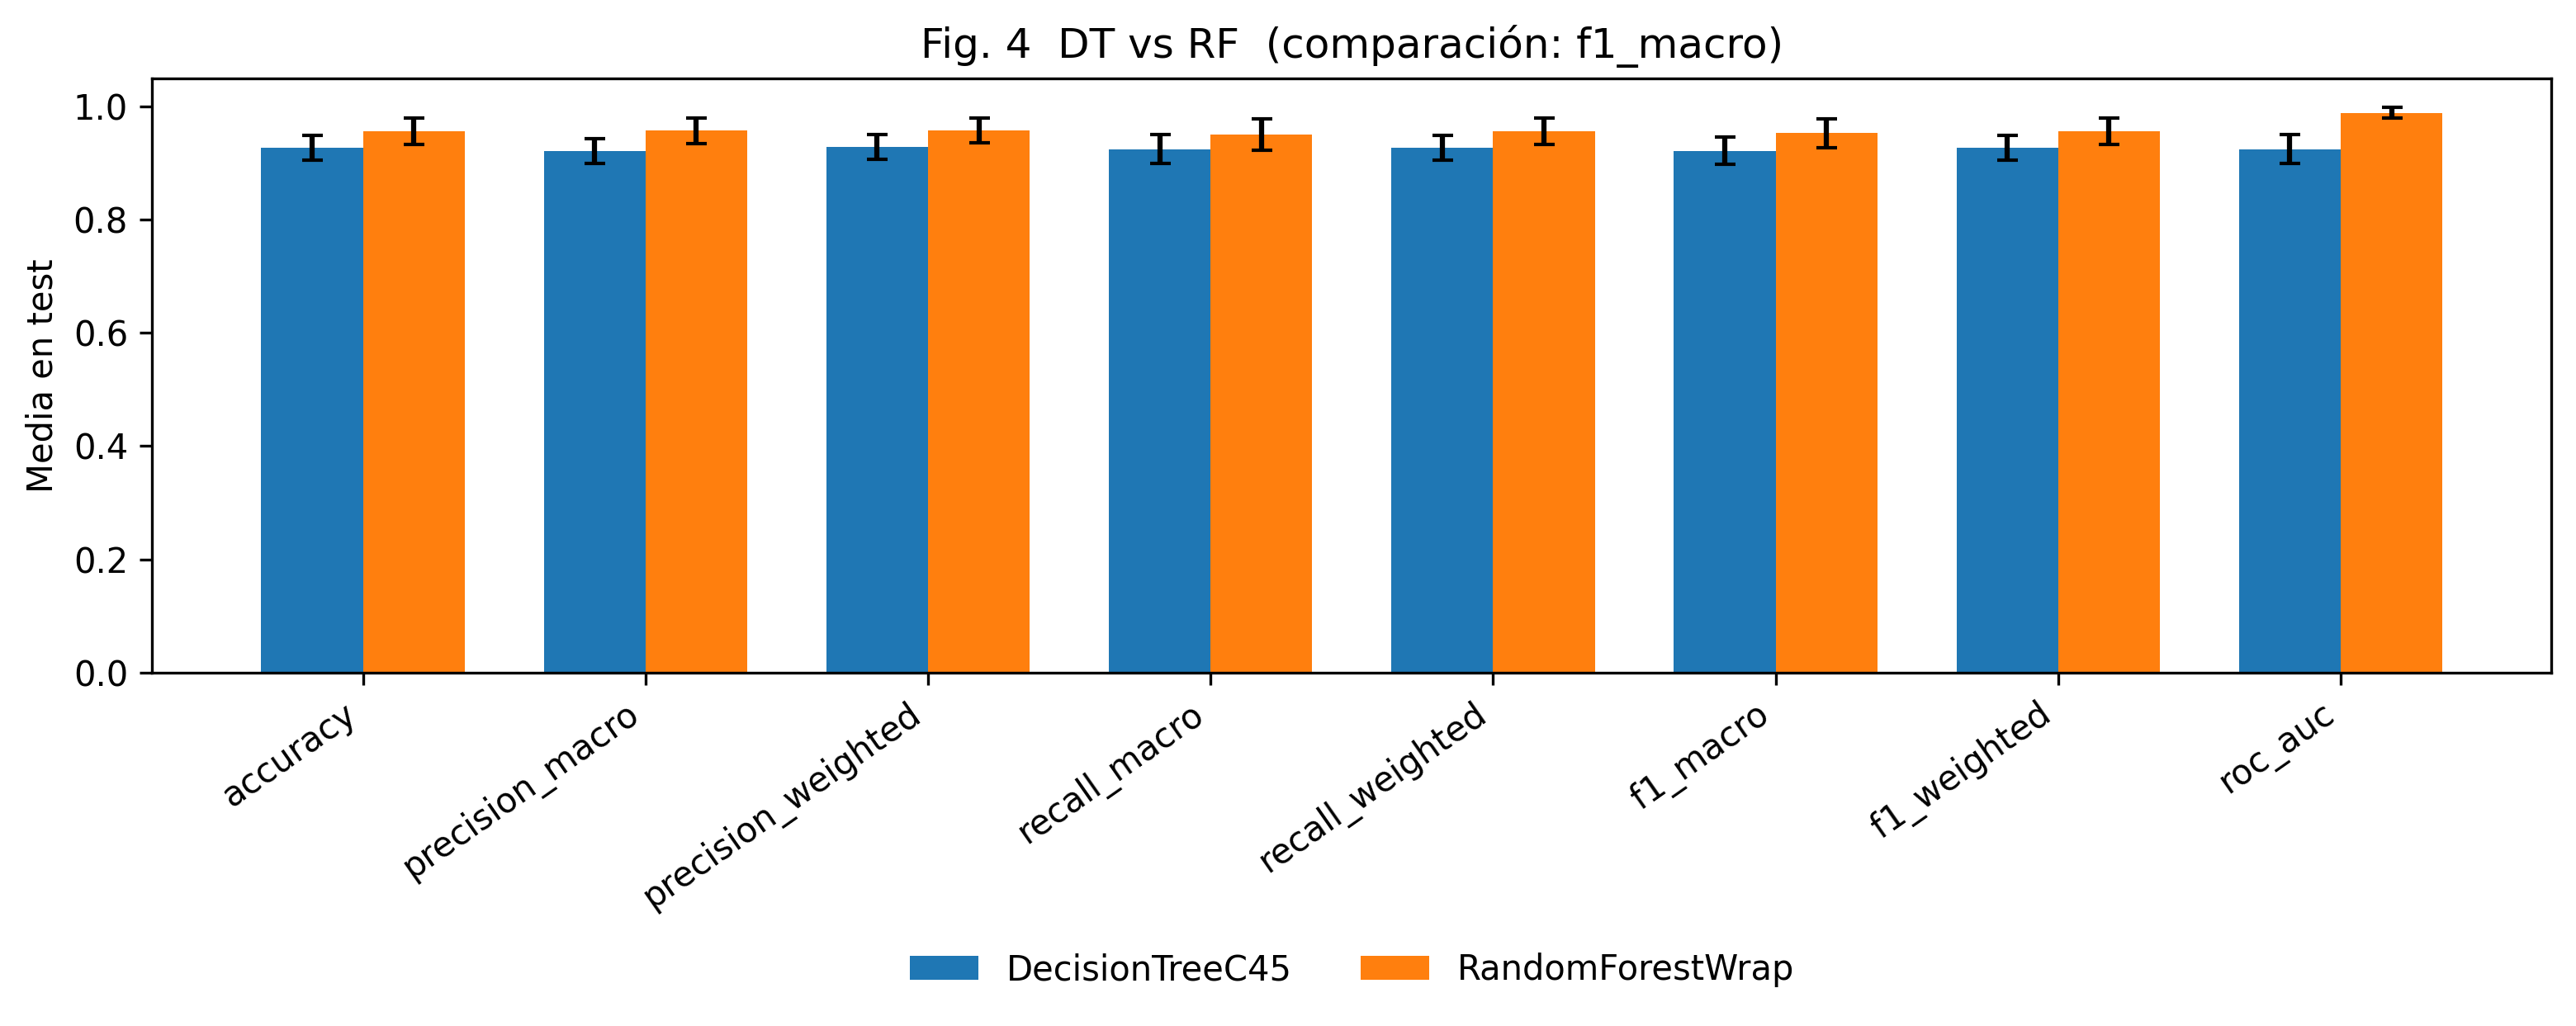
\includegraphics[width=0.92\textwidth]{../figuras/fig4_dt_vs_rf.png}
\caption{Métricas de prueba, media y desvío, en las 25 particiones.}
\label{fig:barras}
\end{figure}

Sin poda el árbol acierta todo el entrenamiento (accuracy 1) y la brecha es 0,0731. Con poda pesimista baja a 30,68 nodos y 15,84 hojas, la accuracy de entrenamiento a 0,9902 y la de prueba sube a 0,9304. La brecha queda en 0,0598. El bosque, sin poda que regularice cada árbol por separado, tiene brecha 0,0436. La baja de 0,0731 a 0,0598 achica el sobreajuste y no llega a una brecha de unos 3 puntos. La Tabla~\ref{tab:poda} y la Figura~\ref{fig:brecha} usan las mismas 25 particiones.

\setcounter{table}{4}
\begin{table}
\caption{DT con poda pesimista y sin poda: media y desvío en 25 particiones.}
\label{tab:poda}
\resizebox{\textwidth}{!}{%
\begin{tabular}{lrrrr}
\toprule
métrica & sin poda media & sin poda desvío & con poda media & con poda desvío \\
\midrule
nodos & 452.0000 & 36.4406 & 71.2000 & 15.7374 \\
hojas & 247.3600 & 18.6299 & 39.0400 & 8.4335 \\
altura & 13.0000 & 0.0000 & 8.8400 & 0.8981 \\
accuracy train & 0.9285 & 0.0086 & 0.8663 & 0.0151 \\
accuracy test & 0.7850 & 0.0265 & 0.7741 & 0.0284 \\
brecha & 0.1435 & 0.0310 & 0.0922 & 0.0353 \\
\bottomrule
\end{tabular}}
\end{table}


\setcounter{figure}{6}
\begin{figure}[ht]
\centering
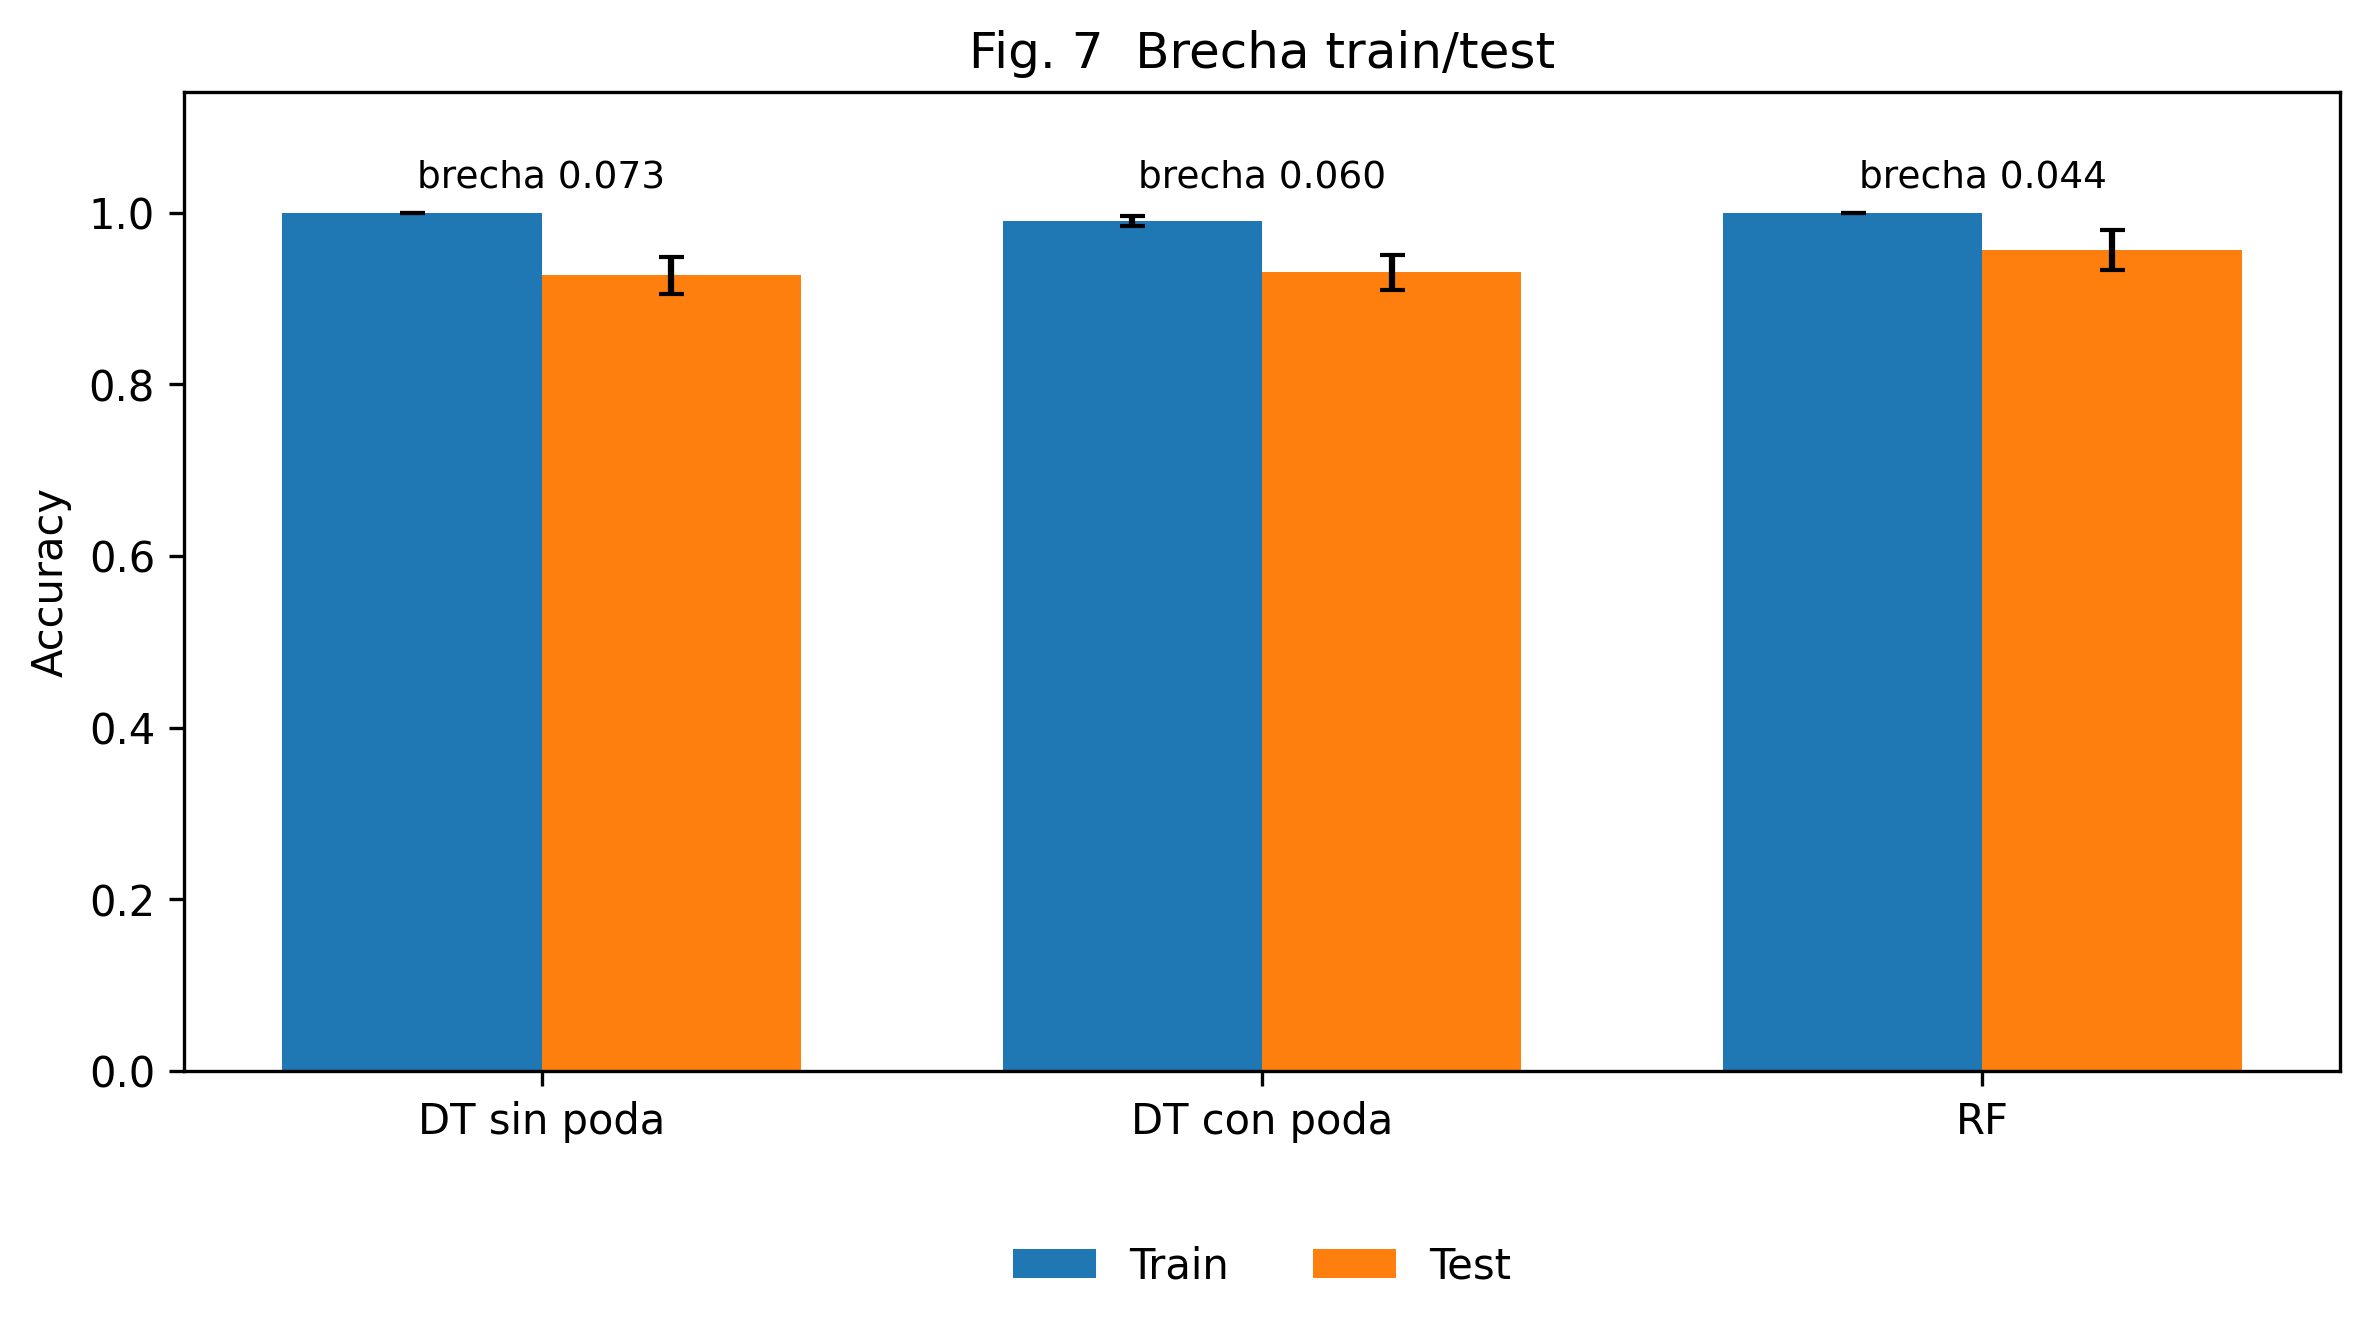
\includegraphics[width=0.78\textwidth]{../figuras/fig7_brecha_train_test.png}
\caption{Accuracy de entrenamiento y de prueba. La brecha es la diferencia de las medias.}
\label{fig:brecha}
\end{figure}

En el holdout, con la positiva \texttt{malignant}, el árbol tiene accuracy 0,9298, F1 macro 0,9246 y ROC-AUC 0,9246. El bosque tiene 0,9737, 0,9713 y 0,9929. La matriz del árbol es 68, 4, 4 y 38 (TN, FP, FN, TP). La del bosque es 72, 0, 3 y 39. En las 114 filas de prueba hay 72 benign y 42 malignant. El árbol se equivoca en 4 de 72 benign (5,6\%) y en 4 de 42 malignant (9,5\%). El bosque no marca ningún benign como malignant y deja pasar 3 de 42 malignant (7,1\%). El árbol reparte el error. El bosque lo concentra en la clase chica. Las Figuras~\ref{fig:confusion} y~\ref{fig:roc} salen de este corte. La matriz de la figura está normalizada por fila.

\setcounter{figure}{8}
\begin{figure}[ht]
\centering
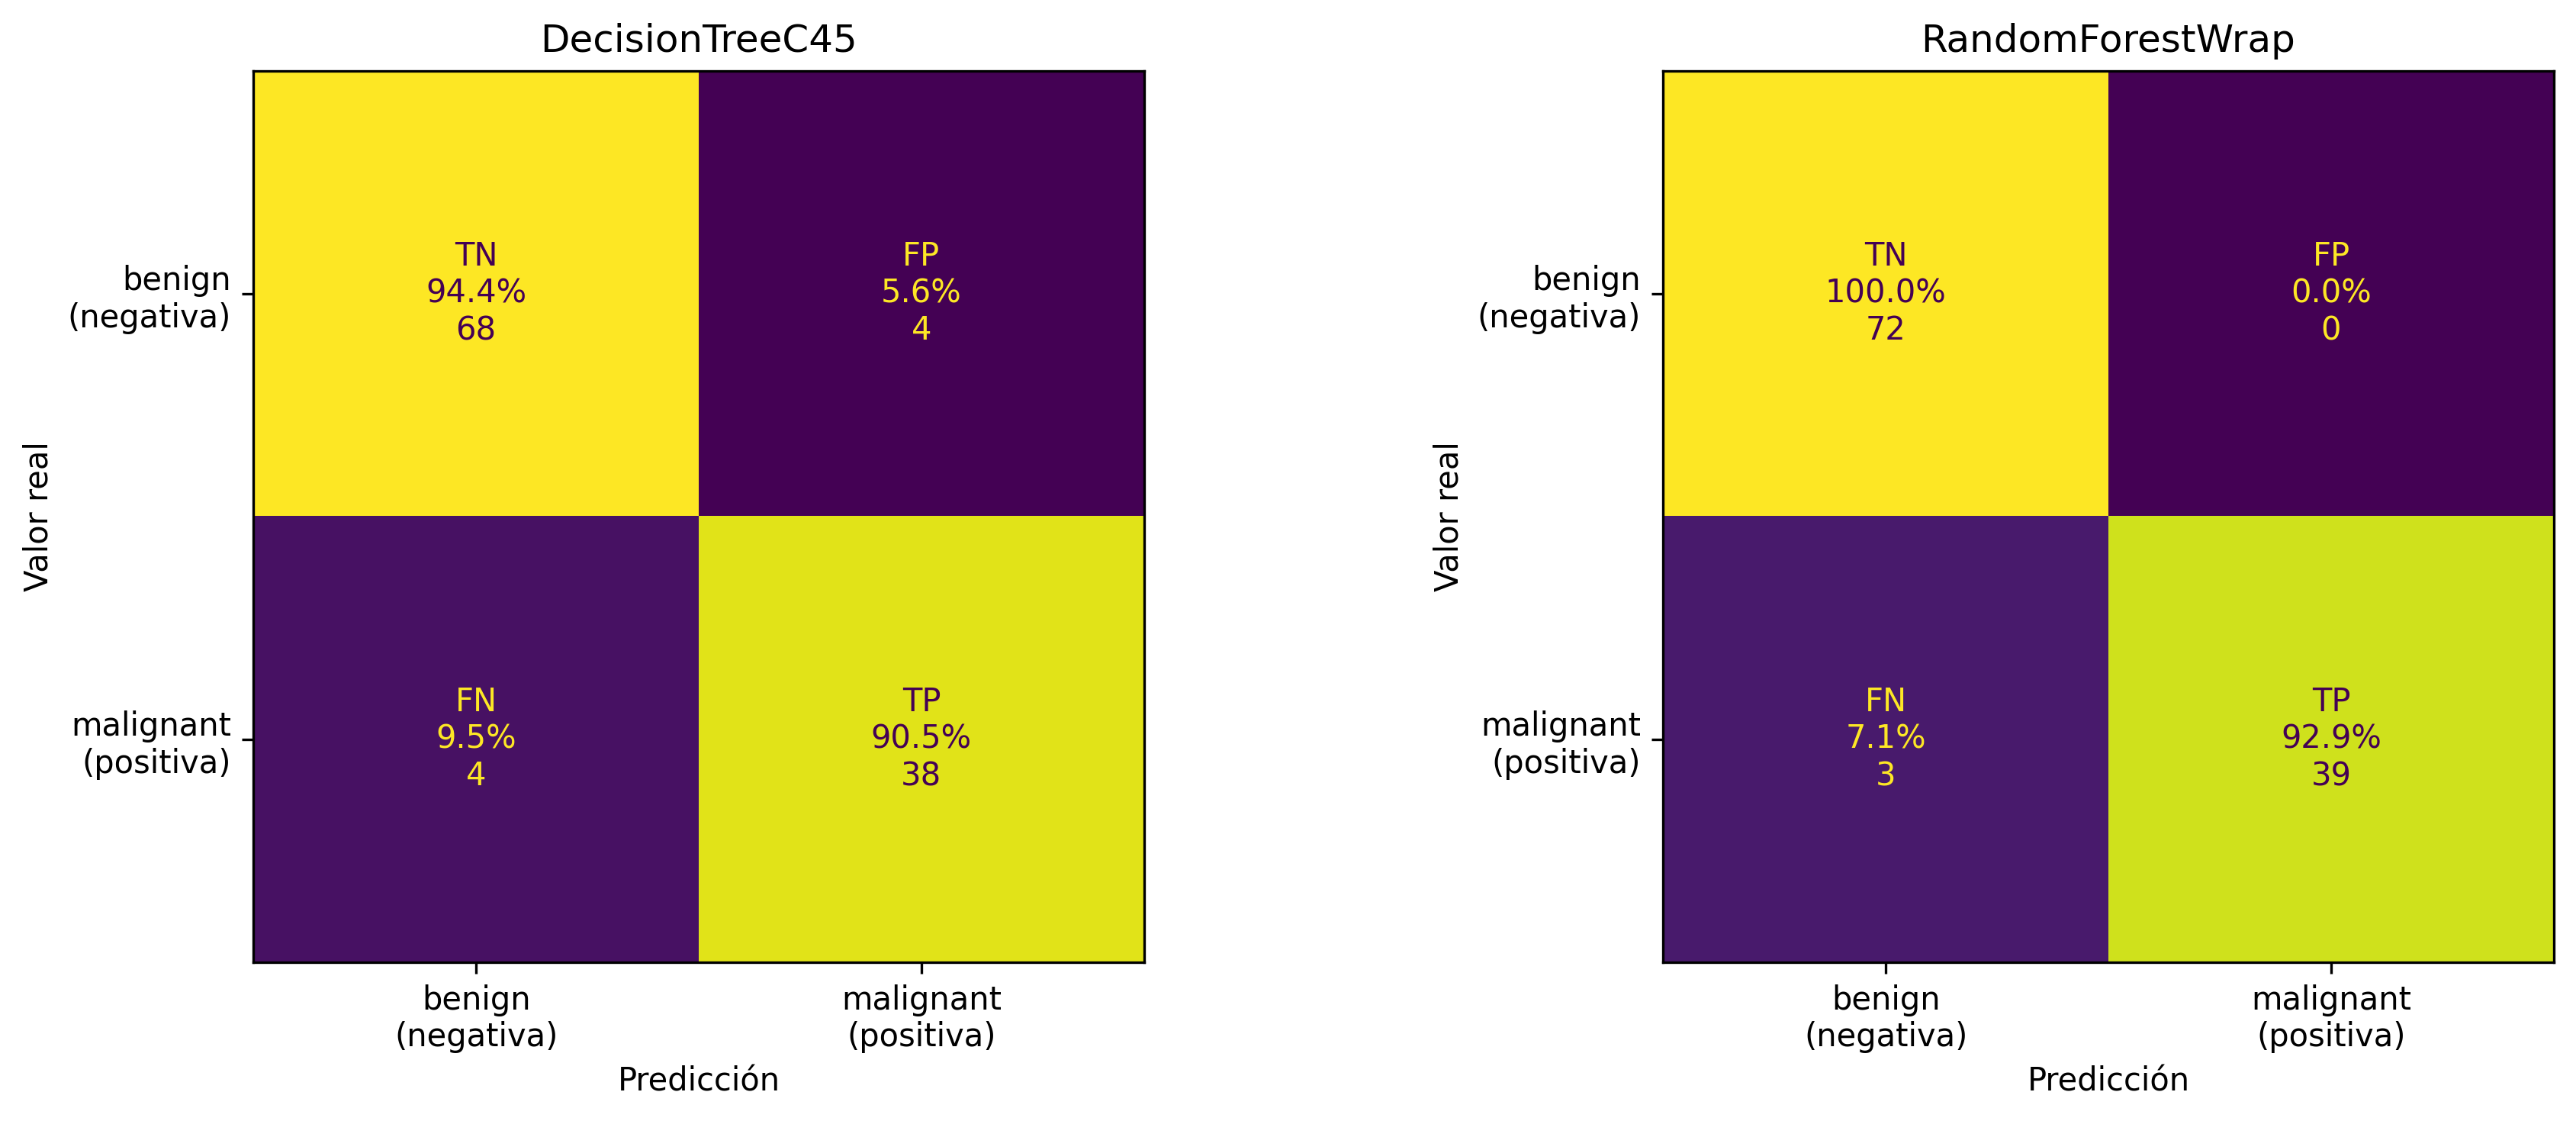
\includegraphics[width=\textwidth]{../figuras/fig9_matrices_confusion.png}
\caption{Matrices de confusión del holdout, normalizadas por fila.}
\label{fig:confusion}
\end{figure}

\setcounter{figure}{9}
\begin{figure}[ht]
\centering
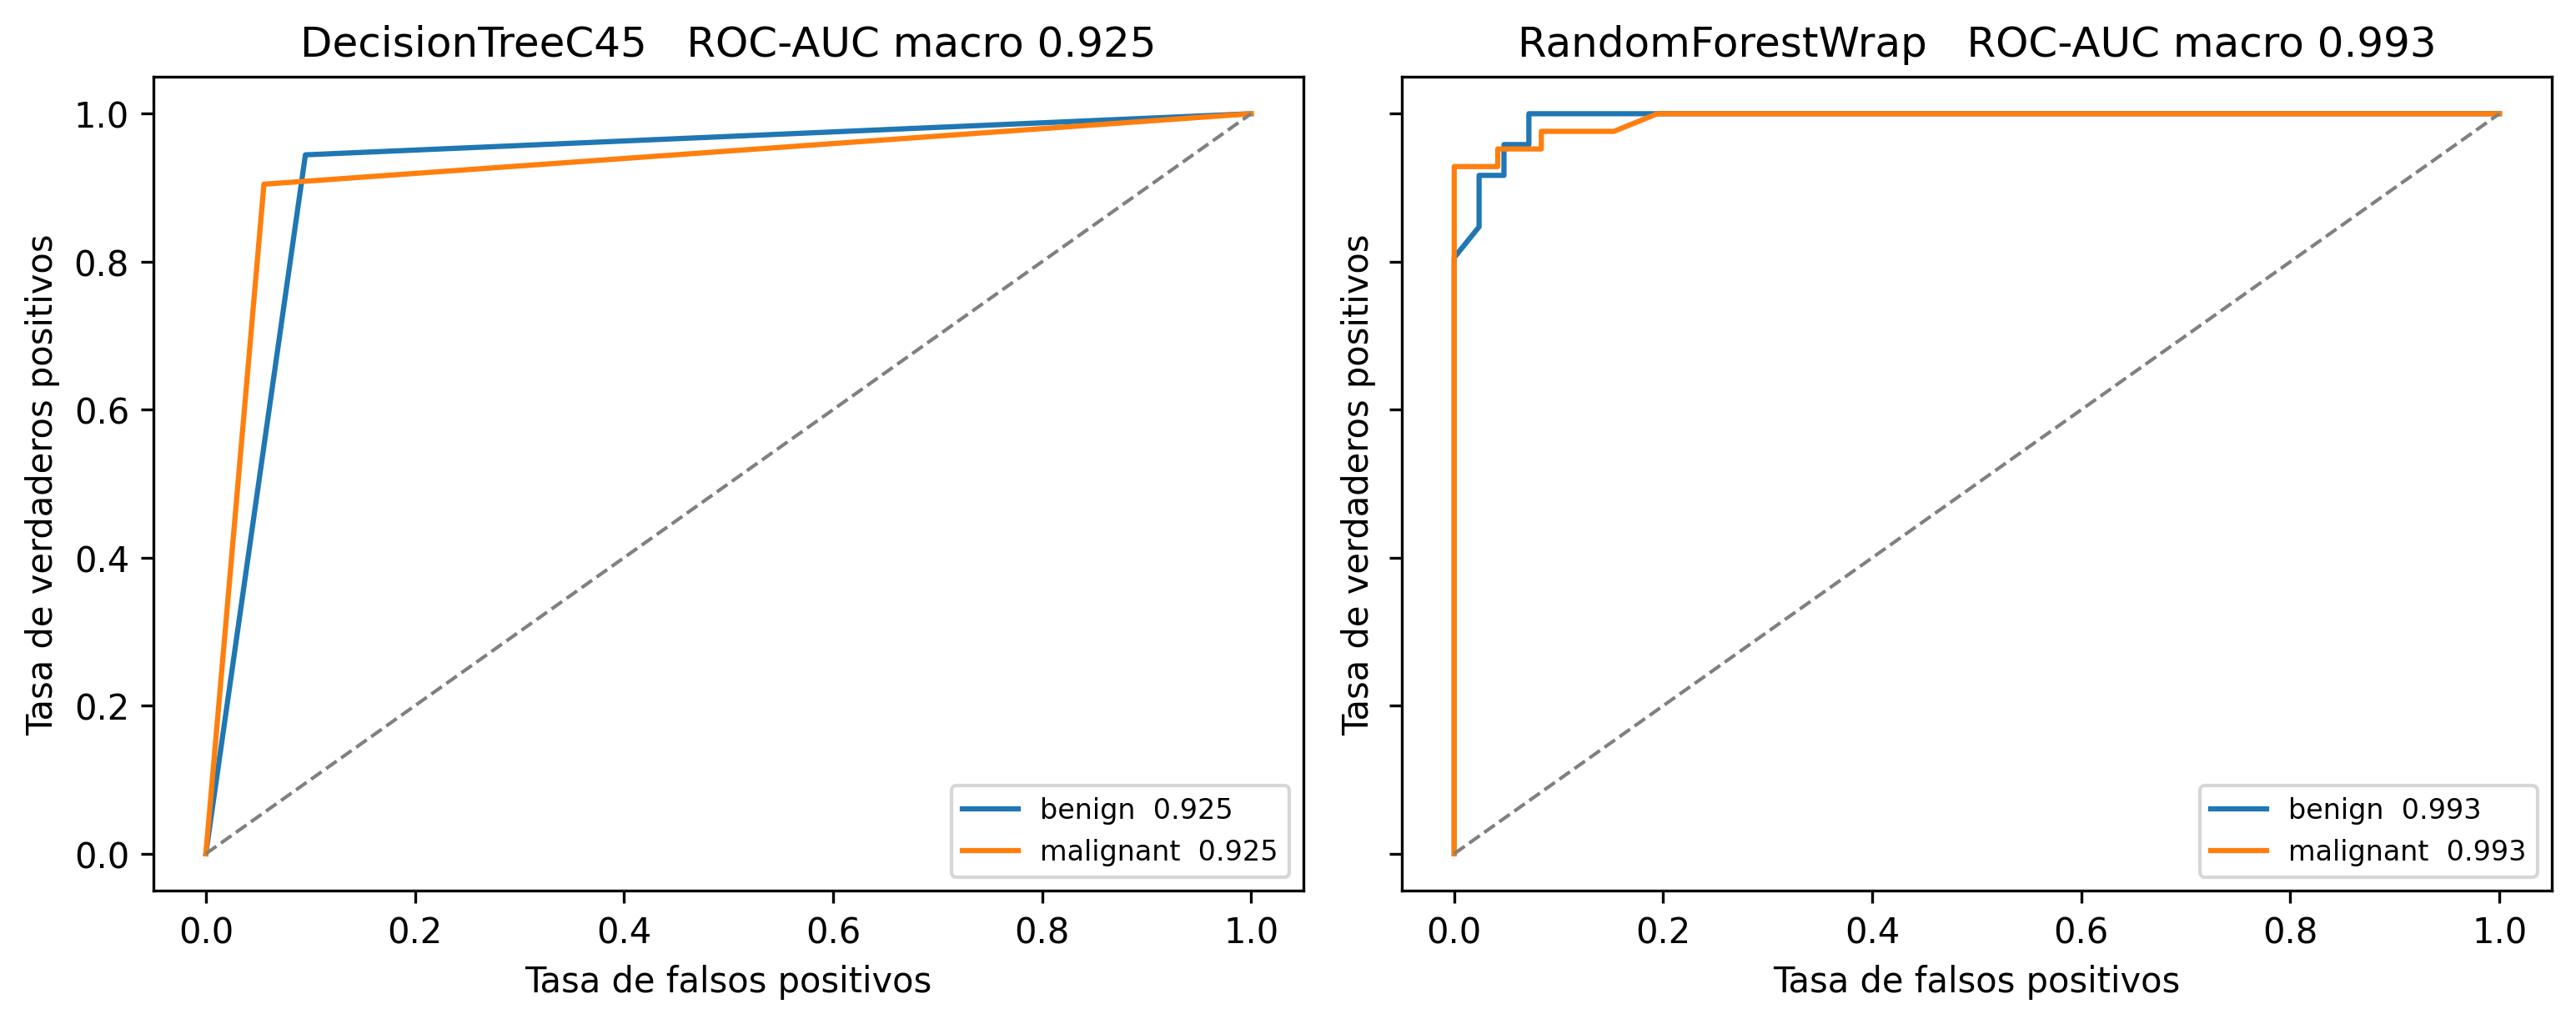
\includegraphics[width=\textwidth]{../figuras/fig10_roc_por_clase.png}
\caption{Curva ROC por clase en el holdout. El título de cada panel es el ROC-AUC macro.}
\label{fig:roc}
\end{figure}

\FloatBarrier
\section{Discusión}
\label{sec:discusion}

Estos números describen un solo dataset de respaldo. No dicen qué va a pasar con el CSV de la cátedra, que puede traer categóricas, faltantes y otra proporción de clases. El manejo fraccional de faltantes y el factor \(t\) quedaron escritos y no tuvieron casos que partir en esta medición.

Tampoco hubo barridos. Profundidad, cantidad de árboles, cantidad de atributos por corte y tamaño mínimo de hoja están en el valor por defecto. Una elección hecha sobre el entrenamiento podría mover la diferencia de F1. Hasta que eso se corra, la comparación es la de las implementaciones con sus valores por defecto.

La poda se juzga por la media de las 25 particiones. En un holdout de la misma semilla, el mismo árbol pasó de 53 a 31 nodos y la accuracy de prueba bajó de 0,9298 a 0,9211. La decisión de podar mira el entrenamiento. Un corte solo no garantiza que el holdout suba, aunque la media de las 25 particiones sí suba de 0,9269 a 0,9304.

El tiempo de ajuste no se lee como una propiedad del algoritmo en abstracto. El árbol está escrito en Python y recorre candidatos en el intérprete. El bosque llama a una implementación compilada. Los 26 segundos frente a 0,19 segundos son el costo medido en esta corrida.

\FloatBarrier
\section{Conclusiones}
\label{sec:conclusiones}

En Breast Cancer Wisconsin, con semilla 42 y sin buscar hiperparámetros, el bosque de scikit-learn supera al árbol del equipo en F1 macro, en accuracy y en ROC-AUC, y se ajusta en una fracción del tiempo. El árbol queda dos órdenes de magnitud más chico.

La poda pesimista con \(\mathit{CF} = 0{,}25\) reduce nodos, hojas, altura y la brecha entre entrenamiento y prueba, y sube un poco la accuracy media de prueba. Eso es un resultado de 25 particiones. En un holdout, la accuracy de prueba puede bajar.

El árbol implementa gain ratio, umbrales continuos, faltantes fraccionarios y la estimación AddErrs. Sigue en deuda con un C4.5 completo en tres puntos ya dichos: un solo corte por atributo continuo, poda sin \emph{subtree raising} y un factor \(t\) propio. Cerrar la comparación pide el dataset de la cátedra y los barridos que todavía no se corrieron.

\bibliographystyle{splncs04}
\bibliography{referencias}

\end{document}
